\documentclass[12pt, a4paper]{article}

% --- Packages ---
\usepackage[utf8]{inputenc}
\usepackage[T1]{fontenc}
\usepackage[english]{babel}
\usepackage{graphicx}
\usepackage{amsmath, amssymb}
\usepackage{booktabs}
\usepackage{hyperref}
\usepackage{geometry}
\usepackage{float}
\usepackage{caption}
\usepackage{subcaption}
\usepackage{algorithm}
\usepackage{algorithmic}
\usepackage{xcolor}
\usepackage{listings}
\usepackage{fancyhdr}

\geometry{margin=2.5cm}

% --- Header/Footer ---
\pagestyle{fancy}
\fancyhf{}
\rhead{Autonomous Robot Navigation}
\lhead{TurtleBot3 - Restaurant Use Case}
\cfoot{\thepage}

% --- Code style ---
\lstset{
  basicstyle=\ttfamily\small,
  keywordstyle=\color{blue},
  commentstyle=\color{gray},
  stringstyle=\color{red},
  frame=single,
  breaklines=true
}

% --- Title ---
\title{
  \vspace{-1cm}
  \textbf{Autonomous Robot Navigation in a Restaurant Environment} \\[0.5cm]
  \large Comparison of Classical Path Planning and Reinforcement Learning \\
  \large with TurtleBot3 in Gazebo/ROS
}
\author{Robotics Project Report}
\date{March 2026}

\begin{document}

\maketitle
\thispagestyle{fancy}

% =====================================================================
\begin{abstract}
This report presents the design and implementation of an autonomous navigation system for a TurtleBot3 robot operating in a simulated restaurant environment. The robot must navigate from a kitchen area to five different table delivery points while avoiding obstacles. Two navigation paradigms are implemented and compared: \textbf{classical path planning} (A*, Dijkstra, and Greedy Best-First Search combined with a Dynamic Window Approach controller) and \textbf{reinforcement learning} (Proximal Policy Optimization, PPO, an Actor-Critic algorithm). The comparison evaluates path efficiency, navigation success rate, obstacle avoidance capabilities, and computation time. Results show that classical planners achieve 100\% reliability with guaranteed obstacle clearance, while the RL agent produces shorter paths but with lower success rates and reduced safety margins.
\end{abstract}

\tableofcontents
\newpage

% =====================================================================
\section{Introduction}

\subsection{Context and Motivation}
The deployment of autonomous mobile robots in service environments such as restaurants, hospitals, and warehouses is a growing field of research. In restaurant settings, robots must navigate safely from a preparation area (kitchen) to customer tables, avoiding static obstacles such as walls, furniture, and other structural elements.

\subsection{Objectives}
The primary objectives of this project are:
\begin{enumerate}
  \item Build a simulated restaurant environment using Gazebo and ROS (Robot Operating System)
  \item Implement classical path planning algorithms (A*, Dijkstra, Greedy) with a DWA controller
  \item Implement a reinforcement learning agent (PPO Actor-Critic) for autonomous navigation
  \item Compare both navigation paradigms on key performance metrics
\end{enumerate}

\subsection{System Overview}
The system operates on a TurtleBot3 Burger platform simulated in Gazebo. The restaurant environment contains walls forming corridors and rooms, with 5 tables as delivery targets. The robot starts from a fixed position in the kitchen area at coordinates $(19.0, 9.0)$ in meters.

% =====================================================================
\section{Environment Setup}

\subsection{Restaurant World Design}
The restaurant environment was designed using Gazebo's SDF format. An aerial photograph of a real restaurant layout was used as reference to create the \texttt{.world} file containing:
\begin{itemize}
  \item Walls forming corridors and rooms (modeled as box geometries)
  \item 5 circular tables (\texttt{cafe\_table} models) positioned in the dining area
  \item A kitchen area where the robot spawns
\end{itemize}

\subsection{Map Generation}
The occupancy grid map was generated using SLAM (Simultaneous Localization and Mapping) with the \texttt{slam\_toolbox} package. Initial attempts using \texttt{explore\_lite} and \texttt{gmapping} failed due to wheel slippage of the TurtleBot3 on smooth surfaces. A dedicated Python script was ultimately used to capture the map reliably.

The resulting map is stored as a PGM (Portable Gray Map) file with the following parameters:
\begin{itemize}
  \item \textbf{Resolution}: $0.05$ m/pixel
  \item \textbf{Origin}: $(-2.0, -2.0, 0.0)$ in world coordinates
  \item \textbf{Occupied threshold}: $0.65$
  \item \textbf{Free threshold}: $0.196$
\end{itemize}

\begin{figure}[H]
  \centering
  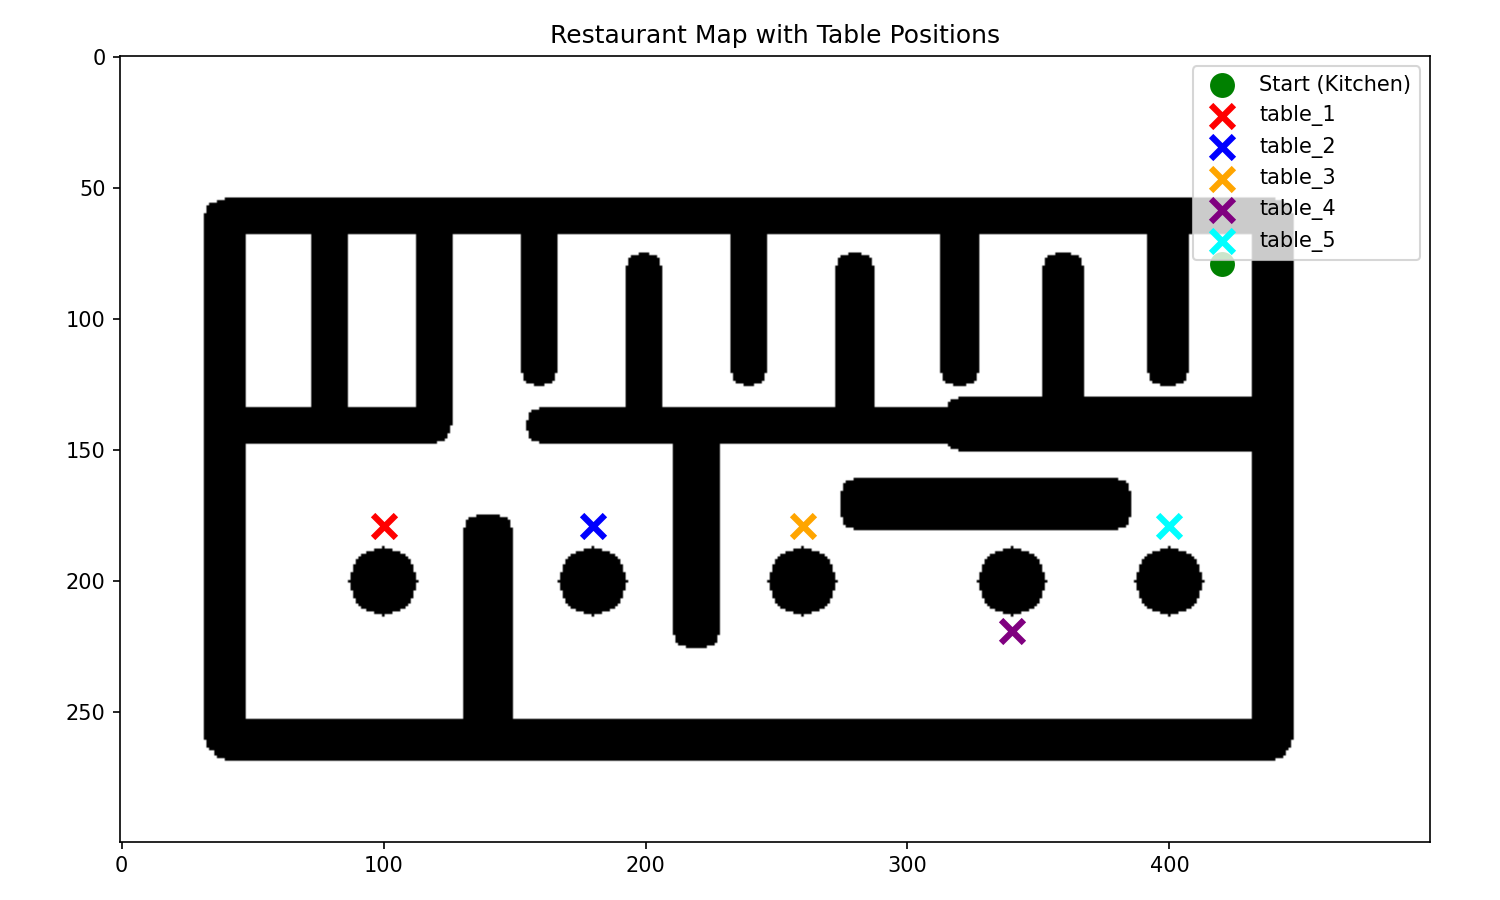
\includegraphics[width=0.85\textwidth]{images/map_tables.png}
  \caption{Restaurant occupancy grid map with the start position (green) and the 5 table delivery points.}
  \label{fig:map_tables}
\end{figure}

\subsection{Coordinate System and Table Positions}
Table coordinates are stored in a JSON configuration file. The coordinate transformation between meters (Gazebo) and pixels (occupancy grid) is:

\begin{equation}
\text{col}_x = \text{round}\left(\frac{x_m - x_{\text{origin}}}{\text{resolution}}\right)
\end{equation}
\begin{equation}
\text{row}_y = (H - 1) - \text{round}\left(\frac{y_m - y_{\text{origin}}}{\text{resolution}}\right)
\end{equation}

where $H$ is the image height in pixels, $(x_{\text{origin}}, y_{\text{origin}})$ is the map origin, and $\text{resolution} = 0.05$ m/pixel.

\begin{table}[H]
\centering
\caption{Table delivery point coordinates (in meters)}
\begin{tabular}{lccc}
\toprule
\textbf{Table ID} & \textbf{X (m)} & \textbf{Y (m)} & \textbf{Description} \\
\midrule
table\_1 & 3.0 & 4.0 & Dining area (left) \\
table\_2 & 7.0 & 4.0 & Dining area (center-left) \\
table\_3 & 11.0 & 4.0 & Dining area (center) \\
table\_4 & 15.0 & 2.0 & Dining area (center-right) \\
table\_5 & 18.0 & 4.0 & Dining area (right) \\
\bottomrule
\end{tabular}
\label{tab:tables}
\end{table}

\subsection{Obstacle Inflation}
To ensure the robot does not collide with walls, obstacle inflation (dilation) is applied to the binary occupancy grid before pathfinding. The inflation radius is computed as:

\begin{equation}
r_{\text{inflation}} = \left\lceil \frac{r_{\text{robot}} + r_{\text{margin}}}{\text{resolution}} \right\rceil \text{ pixels}
\end{equation}

With $r_{\text{robot}} = 0.20$ m and $r_{\text{margin}} = 0.05$ m, this gives $r_{\text{inflation}} = \lceil 5.0 \rceil = 5$ pixels. A circular structuring element is used with SciPy's \texttt{binary\_dilation} function.

% =====================================================================
\section{Classical Navigation}

\subsection{Path Planning Algorithms}

Three classical graph-search algorithms were implemented to find paths on the inflated occupancy grid. All algorithms operate on a 4-connected grid (cardinal neighbors only).

\subsubsection{A* Algorithm}

A* is an informed search algorithm that combines the actual cost $g(n)$ from start to node $n$ with a heuristic estimate $h(n)$ from $n$ to the goal:

\begin{equation}
f(n) = g(n) + h(n)
\end{equation}

The heuristic used is the Manhattan distance:
\begin{equation}
h(n) = |x_n - x_g| + |y_n - y_g|
\end{equation}

A* is \textbf{optimal} and \textbf{complete} when $h(n)$ is admissible (never overestimates the true cost).

\begin{figure}[H]
  \centering
  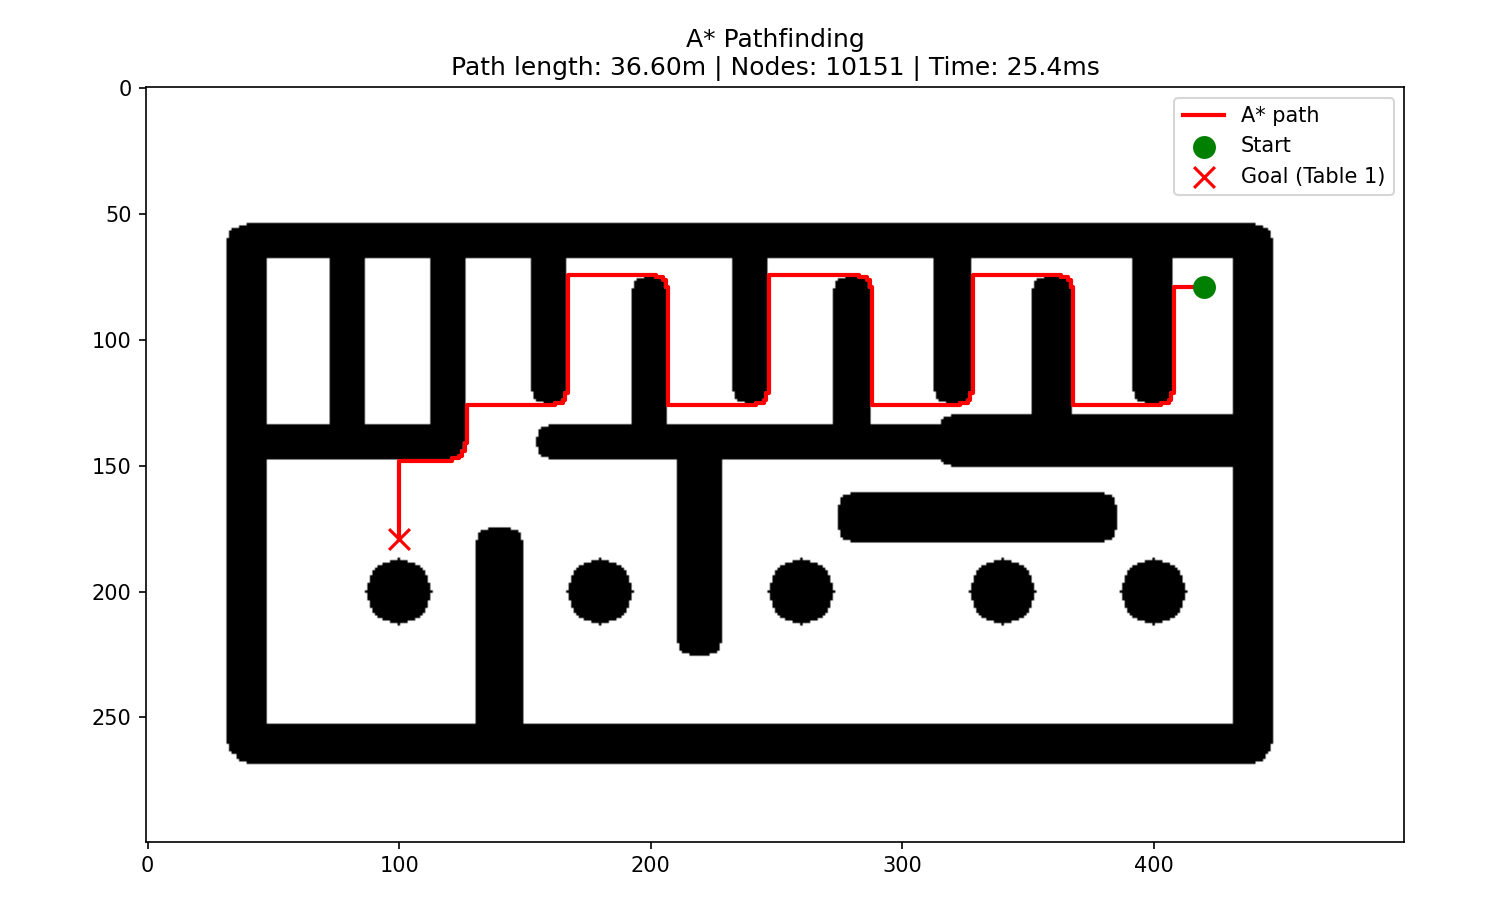
\includegraphics[width=0.85\textwidth]{images/path_astar.png}
  \caption{A* pathfinding result from the kitchen to Table 1.}
  \label{fig:astar}
\end{figure}

\subsubsection{Dijkstra's Algorithm}

Dijkstra's algorithm is a special case of A* with $h(n) = 0$. It explores nodes in order of increasing cost $g(n)$:

\begin{equation}
f(n) = g(n)
\end{equation}

Dijkstra guarantees the optimal path but explores significantly more nodes than A* since it has no directional guidance toward the goal.

\begin{figure}[H]
  \centering
  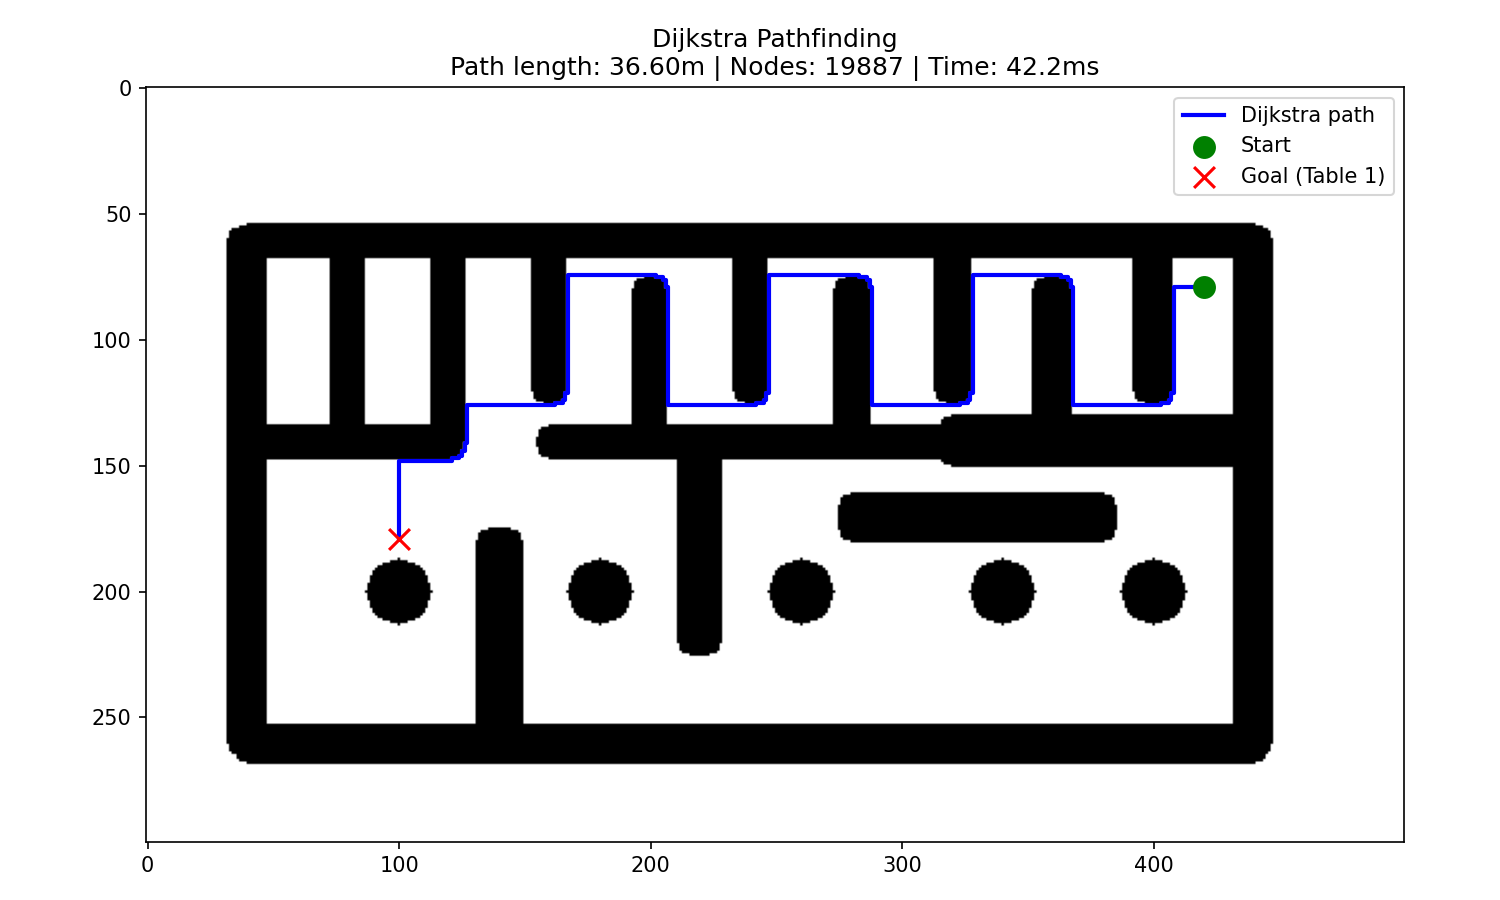
\includegraphics[width=0.85\textwidth]{images/path_dijkstra.png}
  \caption{Dijkstra's pathfinding result from the kitchen to Table 1.}
  \label{fig:dijkstra}
\end{figure}

\subsubsection{Greedy Best-First Search}

Greedy Best-First Search uses only the heuristic to guide the search:

\begin{equation}
f(n) = h(n)
\end{equation}

This makes it the fastest algorithm but \textbf{not optimal}---the path found may be longer than the shortest path. It is also not complete in the presence of certain obstacle configurations.

\begin{figure}[H]
  \centering
  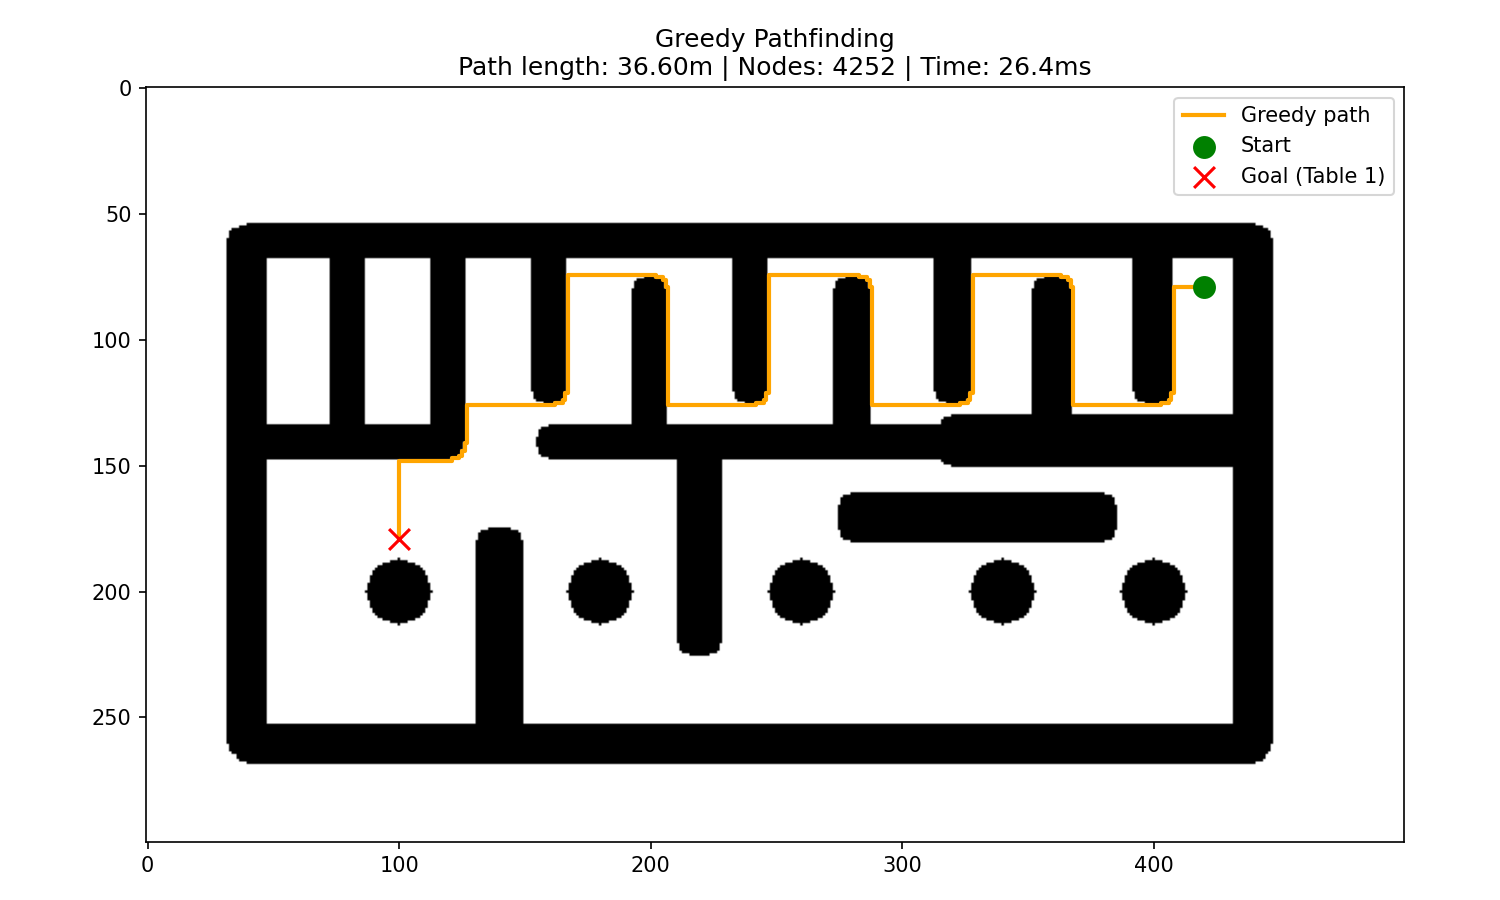
\includegraphics[width=0.85\textwidth]{images/path_greedy.png}
  \caption{Greedy Best-First Search result from the kitchen to Table 1.}
  \label{fig:greedy}
\end{figure}

\subsubsection{Comparison of Path Planning Algorithms}

\begin{figure}[H]
  \centering
  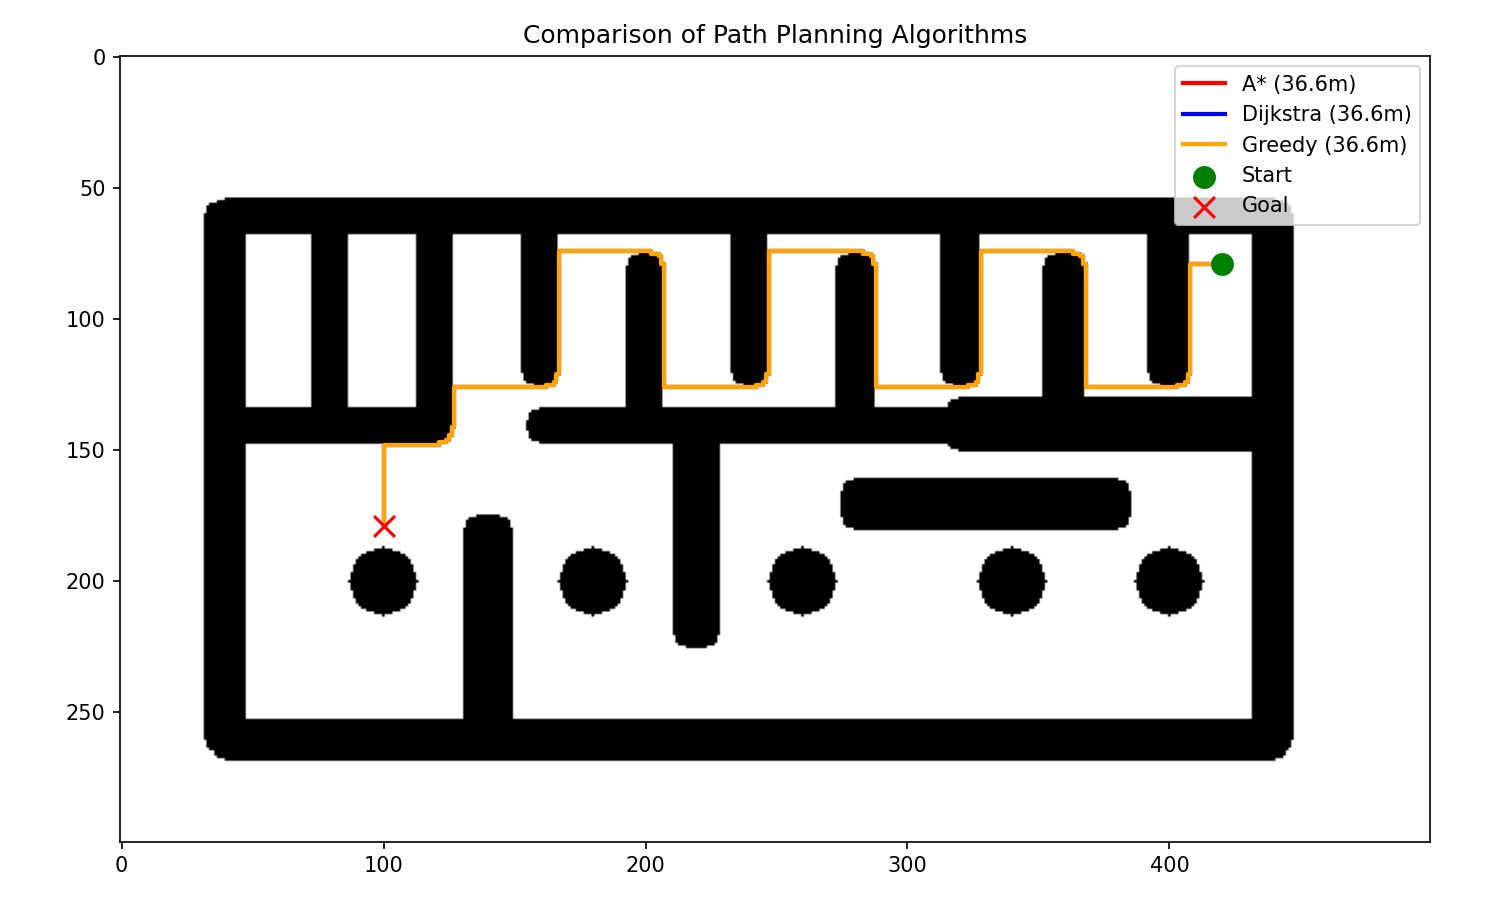
\includegraphics[width=0.85\textwidth]{images/path_comparison.png}
  \caption{Overlay comparison of all three path planning algorithms on the same start-goal pair.}
  \label{fig:path_compare}
\end{figure}

\subsection{DWA Controller (Path Following)}

Once a path is computed, the robot must follow it in the Gazebo simulation. A \textbf{Dynamic Window Approach (DWA)} controller translates the discrete grid path into continuous velocity commands $(v, \omega)$ published on the \texttt{/cmd\_vel} ROS topic.

\subsubsection{Kinematic Model}
The TurtleBot3 is modeled as a differential-drive robot with the unicycle kinematic model:

\begin{equation}
\begin{cases}
x_{t+1} = x_t + v \cos(\theta_t) \cdot \Delta t \\
y_{t+1} = y_t + v \sin(\theta_t) \cdot \Delta t \\
\theta_{t+1} = \theta_t + \omega \cdot \Delta t
\end{cases}
\label{eq:kinematics}
\end{equation}

where $v$ is the linear velocity, $\omega$ is the angular velocity, and $\Delta t = 0.2$ s.

\subsubsection{Dynamic Window}
At each timestep, feasible velocities are constrained by the robot's acceleration limits:

\begin{equation}
V_s = \{(v, \omega) \mid v \in [v_c - a_v \Delta t,\ v_c + a_v \Delta t],\ \omega \in [\omega_c - a_\omega \Delta t,\ \omega_c + a_\omega \Delta t]\}
\end{equation}

with $v_{\max} = 0.5$ m/s, $\omega_{\max} = 1.0$ rad/s, $a_v = 0.5$ m/s$^2$, and $a_\omega = 1.0$ rad/s$^2$.

\subsubsection{Cost Function}
Each candidate trajectory $(v, \omega)$ is evaluated over a prediction horizon of $H = 5$ steps using:

\begin{equation}
J(v, \omega) = \alpha \cdot d_{\text{path}} + \beta \cdot \Delta\theta_{\text{heading}} + \gamma \cdot (v_{\max} - v)
\end{equation}

where:
\begin{itemize}
  \item $d_{\text{path}}$: minimum distance from the simulated endpoint to the reference path ($\alpha = 2.0$)
  \item $\Delta\theta_{\text{heading}}$: angular difference to the lookahead point on the path ($\beta = 1.0$)
  \item $(v_{\max} - v)$: velocity reward to encourage forward motion ($\gamma = 0.5$)
\end{itemize}

The velocity pair $(v^*, \omega^*) = \arg\min J(v, \omega)$ is selected and published.

% =====================================================================
\section{Reinforcement Learning Navigation}

\subsection{Problem Formulation as MDP}

The navigation task is formulated as a Markov Decision Process (MDP):
\begin{itemize}
  \item \textbf{State space} $\mathcal{S}$: 26-dimensional continuous vector
  \item \textbf{Action space} $\mathcal{A}$: 2-dimensional continuous box $[0, 0.5] \times [-1.0, 1.0]$
  \item \textbf{Reward function} $R(s, a)$: shaped reward (see Section~\ref{sec:reward})
  \item \textbf{Discount factor} $\gamma = 0.99$
\end{itemize}

\subsection{Environment: FastRobot2DEnv}

A custom Gymnasium environment (\texttt{FastRobot2DEnv}) was implemented for fast training without Gazebo overhead. It uses the same occupancy grid and coordinate transformations as the classical planners.

\subsubsection{Observation Space (26 values)}

The observation vector consists of:

\begin{enumerate}
  \item \textbf{Simulated LiDAR (24 rays)}: 24 distance measurements uniformly distributed over $[-\pi, \pi]$ (one ray every $15°$). Each ray is computed via raycasting on the occupancy grid:
  \begin{equation}
  d_i = \min\left(d_{\max},\ \min_{k} \left\{ k \cdot \frac{\text{res}}{2} : \text{grid}\left[\text{pos} + k \cdot \frac{\text{res}}{2} \cdot \vec{u}_i\right] = \text{obstacle} \right\}\right)
  \end{equation}
  where $\vec{u}_i = (\cos(\theta + \alpha_i), \sin(\theta + \alpha_i))$ and $d_{\max} = 3.5$ m.

  \item \textbf{True distance (1 value)}: The geodesic distance to the goal computed from a pre-computed \textbf{distance map} (see Section~\ref{sec:distmap}).

  \item \textbf{Heading angle (1 value)}: Relative angle from the robot's orientation to the goal:
  \begin{equation}
  \phi = \text{atan2}(y_g - y_r,\ x_g - x_r) - \theta_r
  \end{equation}
  normalized to $[-\pi, \pi]$.
\end{enumerate}

\subsubsection{Action Space}

The action is a 2D continuous vector:
\begin{equation}
a = (v, \omega) \in [0.0, 0.5] \times [-1.0, 1.0]
\end{equation}

where $v$ is linear velocity (m/s) and $\omega$ is angular velocity (rad/s).

\subsubsection{Distance Map (Dijkstra Flood Fill)}
\label{sec:distmap}

Instead of using Euclidean distance as reward signal (which ignores walls), a \textbf{distance map} is pre-computed for each table using a BFS/Dijkstra flood-fill from the goal position. This provides the true shortest-path distance to the goal at every grid cell:

\begin{equation}
D(r, c) = \min_{\text{path}} \sum_{i} w_i
\end{equation}

where $w_i = 1.0$ for cardinal moves and $w_i = \sqrt{2} \approx 1.414$ for diagonal moves. Obstacle cells retain the value $D = 9999$ (unreachable).

The distance maps for all 5 tables are pre-computed once during initialization, making each \texttt{reset()} call $O(1)$ instead of $O(W \times H)$.

\subsection{Reward Function}
\label{sec:reward}

The reward function is designed to guide the agent toward the goal efficiently:

\begin{equation}
R(s_t, a_t) = 
\begin{cases}
+2000 & \text{if } \|p_{\text{robot}} - p_{\text{goal}}\|_2 < 0.35 \text{ m (success)} \\
-500 & \text{if collision with obstacle (crash)} \\
\underbrace{50 \cdot (D_{t-1} - D_t)}_{\text{progress}} - \underbrace{0.5}_{\text{time penalty}} - \underbrace{0.3 \cdot |\omega_t|}_{\text{rotation penalty}} & \text{otherwise}
\end{cases}
\end{equation}

where $D_t$ is the geodesic distance at time $t$ (from the distance map, in meters).

Key design decisions:
\begin{itemize}
  \item \textbf{Progress reward}: Uses the Dijkstra distance map instead of Euclidean distance, ensuring the robot is rewarded for following the actual shortest path through corridors.
  \item \textbf{Time penalty}: Encourages the robot to find short paths, preventing indefinite wandering.
  \item \textbf{Rotation penalty}: Penalizes excessive turning, producing smoother trajectories. Without this, the robot tends to oscillate (zigzag) in corridors.
  \item \textbf{Asymmetric terminal rewards}: The success reward (+2000) significantly exceeds the maximum cumulative penalty, ensuring the agent always prefers reaching the goal over ``suiciding'' into a wall.
\end{itemize}

\subsection{PPO Algorithm (Actor-Critic)}

\textbf{Proximal Policy Optimization (PPO)} is a policy gradient method that uses an Actor-Critic architecture:

\begin{itemize}
  \item \textbf{Actor} $\pi_\theta(a|s)$: A neural network that outputs a Gaussian distribution over actions.
  \item \textbf{Critic} $V_\phi(s)$: A neural network that estimates the value function (expected cumulative reward from state $s$).
\end{itemize}

\subsubsection{Policy Loss (Actor)}

PPO clips the policy update to prevent catastrophically large changes:

\begin{equation}
L^{\text{CLIP}}(\theta) = \mathbb{E}_t \left[ \min\left( r_t(\theta) \hat{A}_t,\ \text{clip}(r_t(\theta), 1 - \epsilon, 1 + \epsilon) \hat{A}_t \right) \right]
\end{equation}

where $r_t(\theta) = \frac{\pi_\theta(a_t | s_t)}{\pi_{\theta_{\text{old}}}(a_t | s_t)}$ is the probability ratio, $\hat{A}_t$ is the Generalized Advantage Estimate (GAE), and $\epsilon = 0.2$ is the clip range.

\subsubsection{Value Loss (Critic)}

\begin{equation}
L^{\text{VF}}(\phi) = \mathbb{E}_t \left[ \left( V_\phi(s_t) - V_t^{\text{target}} \right)^2 \right]
\end{equation}

\subsubsection{Entropy Bonus}

An entropy term encourages exploration:
\begin{equation}
H(\pi_\theta) = -\mathbb{E}[\log \pi_\theta(a|s)]
\end{equation}

\subsubsection{Total Loss}

\begin{equation}
L(\theta, \phi) = -L^{\text{CLIP}}(\theta) + c_1 \cdot L^{\text{VF}}(\phi) - c_2 \cdot H(\pi_\theta)
\end{equation}

with $c_1 = 0.5$ and $c_2 = 0.01$ (entropy coefficient).

\subsubsection{Training Hyperparameters}

\begin{table}[H]
\centering
\caption{PPO Training Hyperparameters}
\begin{tabular}{lc}
\toprule
\textbf{Parameter} & \textbf{Value} \\
\midrule
Algorithm & PPO (Stable-Baselines3) \\
Network architecture & MLP (2 hidden layers, 64 neurons each) \\
Learning rate & $1 \times 10^{-4}$ \\
Rollout steps ($n_{\text{steps}}$) & 4096 \\
Batch size & 128 \\
Clip range ($\epsilon$) & 0.2 \\
Entropy coefficient ($c_2$) & 0.01 \\
Target KL divergence & 0.015 \\
Total timesteps & 1,000,000 \\
Discount factor ($\gamma$) & 0.99 \\
Episode timeout & 1500 steps (150 s) \\
Device & CPU \\
\bottomrule
\end{tabular}
\label{tab:hyperparams}
\end{table}

\subsection{Training Results}

\begin{figure}[H]
  \centering
  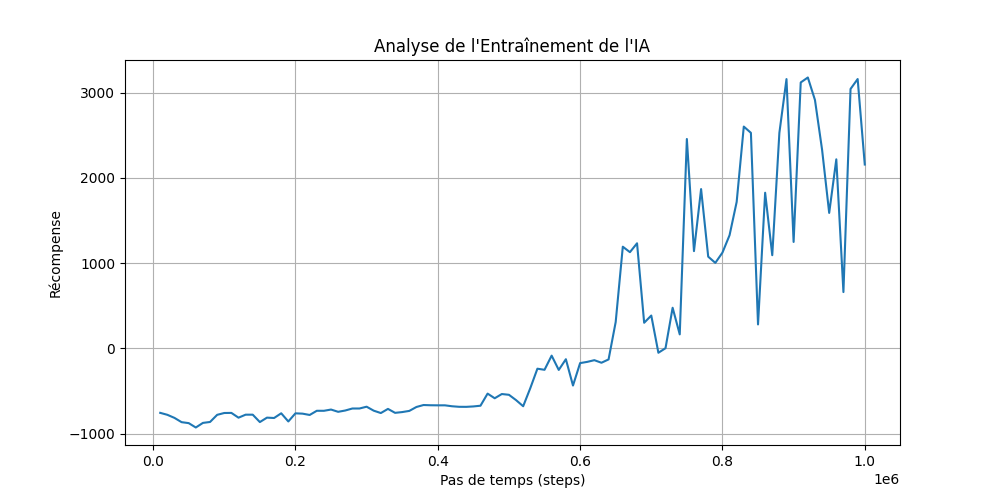
\includegraphics[width=0.85\textwidth]{images/resultats_entrainement_final.png}
  \caption{Training curve of the PPO agent. Mean evaluation reward over timesteps. The agent reaches stable positive rewards around $\sim$3000 after approximately 500,000 timesteps.}
  \label{fig:training_curve}
\end{figure}

\subsection{IA Navigation Trajectories}

\begin{figure}[H]
  \centering
  
\includegraphics[width=0.85\textwidth]{images/resultat_ia_test.png}
  \caption{RL agent trajectories to different tables. The agent successfully navigates through corridors, demonstrating learned obstacle avoidance behavior.}
  \label{fig:ia_trajectories}
\end{figure}

% =====================================================================
\section{Comparative Analysis}

\subsection{Benchmark Methodology}

Both navigation paradigms were tested on all 5 tables from the same starting position $(19.0, 9.0)$. For classical planners, each algorithm was run once per table (deterministic). For the RL agent, 5 trials per table were conducted to measure variability and success rate.

\subsection{Results}

\begin{figure}[H]
  \centering
  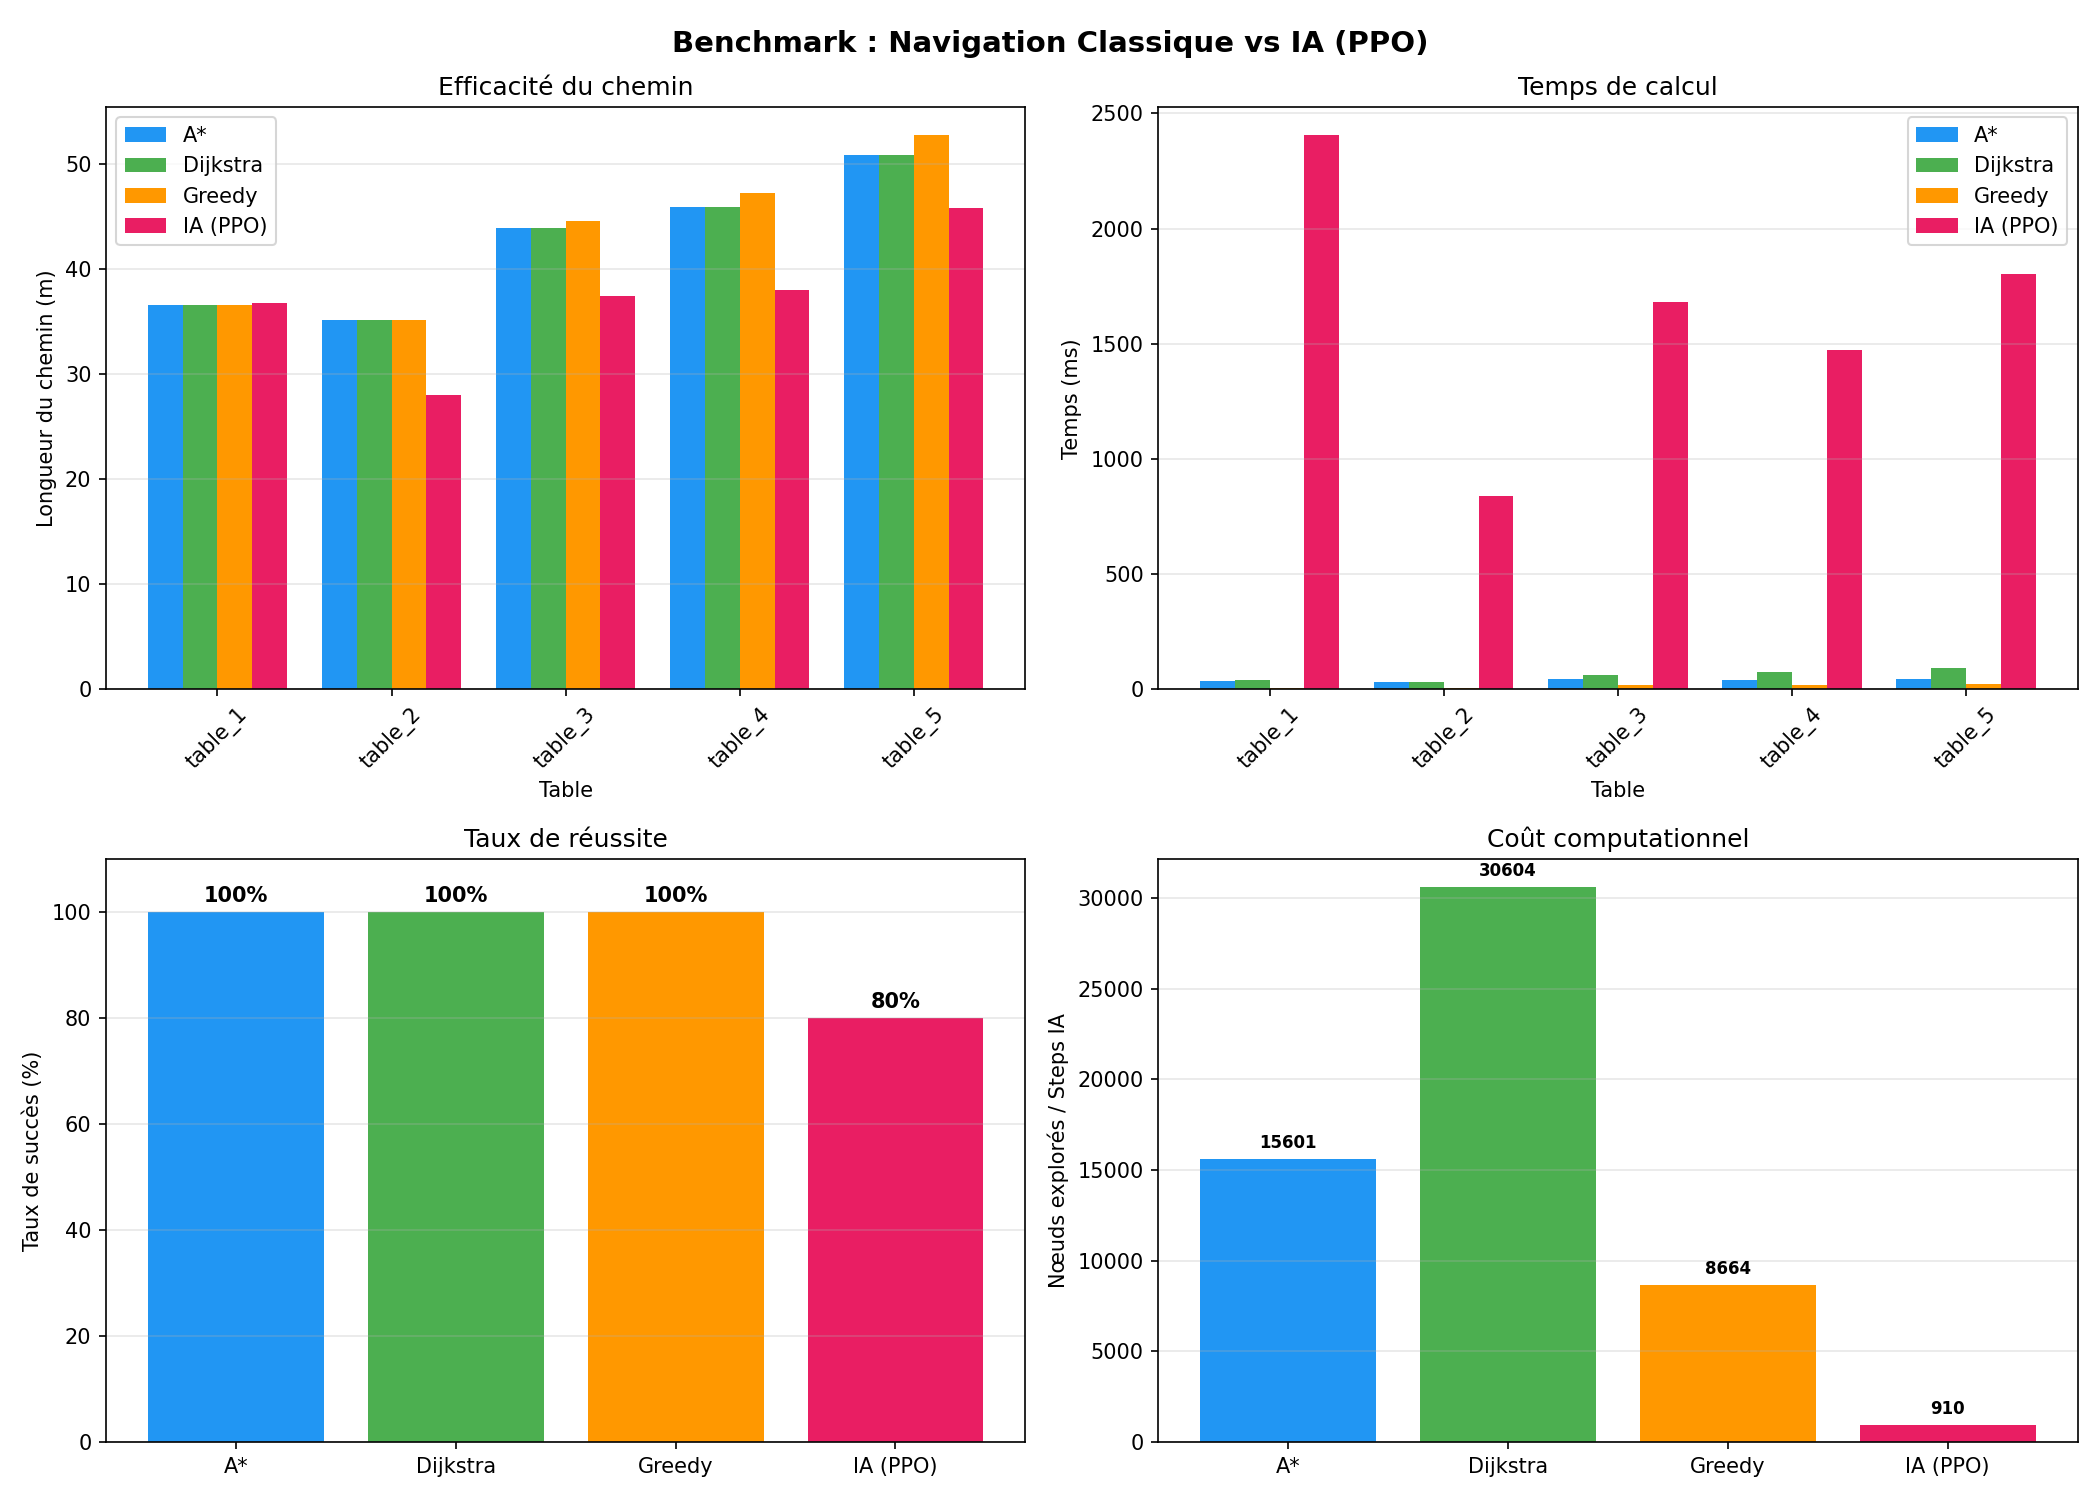
\includegraphics[width=\textwidth]{images/benchmark_comparaison.png}
  \caption{Comprehensive benchmark comparing classical path planning (A*, Dijkstra, Greedy) and RL navigation (PPO) across four metrics.}
  \label{fig:benchmark}
\end{figure}

\begin{table}[H]
\centering
\caption{Quantitative comparison of navigation approaches (averaged over all 5 tables)}
\begin{tabular}{lcccc}
\toprule
\textbf{Metric} & \textbf{A*} & \textbf{Dijkstra} & \textbf{Greedy} & \textbf{IA (PPO)} \\
\midrule
Success rate (\%) & \textbf{100} & \textbf{100} & \textbf{100} & 80 \\
Mean path length (m) & 42.50 & 42.50 & 43.30 & \textbf{37.23} \\
Mean computation time (ms) & 40.8 & 60.3 & \textbf{15.3} & 1641.4 \\
Mean nodes explored / steps & 15,601 & 30,604 & 8,664 & \textbf{910} \\
Min. obstacle distance (m) & $\geq 0.25$ & $\geq 0.25$ & $\geq 0.25$ & 0.04 \\
Crashes & 0 & 0 & 0 & 0 \\
\bottomrule
\end{tabular}
\label{tab:benchmark}
\end{table}

\subsection{Analysis}

\subsubsection{Path Efficiency}
The RL agent produces \textbf{shorter paths} (37.23 m vs.\ 42.50 m for A*/Dijkstra), a 12.4\% improvement. This is because the RL agent operates in continuous space and can take diagonal trajectories and smooth curves, whereas grid-based planners are restricted to 4-connected cardinal movements (up, down, left, right), introducing unnecessary Manhattan-style detours.

\subsubsection{Navigation Success Rate}
Classical planners achieve a \textbf{perfect 100\% success rate}. They are deterministic algorithms with mathematical guarantees of completeness (A* and Dijkstra). The RL agent achieves 80\% success rate, failing occasionally on certain table configurations. This is inherent to the stochastic nature of the learned policy and could be improved with additional training or curriculum learning.

\subsubsection{Obstacle Avoidance}
Classical planners use \textbf{obstacle inflation} (25 cm clearance), providing a hard safety guarantee. The robot \emph{cannot} approach walls closer than this margin. The RL agent, however, navigates as close as \textbf{4 cm} to obstacles. While no crashes occurred during testing, this margin is dangerously small for real-world deployment.

\subsubsection{Computation Time}
Classical planners are \textbf{40--100$\times$ faster} than the RL agent at inference time. A* takes 40.8 ms, Greedy only 15.3 ms, while the RL agent requires 1641 ms per trajectory. However, this comparison excludes the RL \textbf{training time} ($\sim$30 minutes for 1M timesteps), which is a one-time offline cost.

\subsubsection{Computational Resources}

\begin{table}[H]
\centering
\caption{Resource requirements for each approach}
\begin{tabular}{lcc}
\toprule
\textbf{Resource} & \textbf{Classical (A* + DWA)} & \textbf{RL (PPO)} \\
\midrule
Training time & None (no training) & $\sim$30 min (offline) \\
Inference time per path & $\sim$40 ms & $\sim$1.6 s \\
Memory (runtime) & $\sim$50 MB (grid) & $\sim$200 MB (model + grid) \\
Dependencies & NumPy, SciPy & PyTorch, Gymnasium, SB3 \\
GPU required & No & No (CPU sufficient) \\
\bottomrule
\end{tabular}
\end{table}

% =====================================================================
\section{Discussion}

\subsection{Strengths and Weaknesses}

\begin{table}[H]
\centering
\caption{Summary of strengths and weaknesses}
\begin{tabular}{p{3.5cm}p{5cm}p{5cm}}
\toprule
\textbf{Criterion} & \textbf{Classical Navigation} & \textbf{RL Navigation} \\
\midrule
\textbf{Reliability} & Deterministic, guaranteed & Stochastic, may fail \\
\textbf{Path quality} & Optimal (A*, Dijkstra) & Shorter but variable \\
\textbf{Safety} & Hard safety margins & Learned, no guarantee \\
\textbf{Adaptability} & Requires re-planning & Adapts via policy \\
\textbf{Setup effort} & Algorithm selection & Training + reward shaping \\
\textbf{Generalization} & Map-specific & Can generalize to new maps \\
\bottomrule
\end{tabular}
\end{table}

\subsection{Potential Improvements for the RL Agent}
\begin{itemize}
  \item \textbf{Curriculum learning}: Start training with nearby goals and progressively increase difficulty.
  \item \textbf{Reward shaping}: Increase the time penalty further to produce shorter paths.
  \item \textbf{Safety layer}: Add a hard constraint that overrides RL actions when too close to obstacles.
  \item \textbf{More training}: The model plateaus around 1M steps; domain randomization and longer training could improve generalization.
  \item \textbf{Sim-to-real transfer}: The 2D simulation does not model real-world noise, sensor inaccuracies, or wheel slippage.
\end{itemize}

% =====================================================================
\section{Conclusion}

This project demonstrates the implementation and comparison of two fundamentally different approaches to autonomous robot navigation in a restaurant environment. Classical path planning with DWA control provides a \textbf{reliable, fast, and safe} solution that is immediately deployable. Reinforcement learning using PPO Actor-Critic produces \textbf{shorter, smoother paths} but at the cost of reduced reliability and safety margins.

For a production restaurant robot, a \textbf{hybrid approach} would be ideal: use classical planning for path computation (guaranteed safety) and RL for local control refinement (smoother trajectories). The RL agent's ability to produce continuous velocity commands naturally complements the discrete grid paths produced by classical planners.

\begin{thebibliography}{9}
\bibitem{ppo} Schulman, J., et al. ``Proximal Policy Optimization Algorithms.'' \textit{arXiv:1707.06347}, 2017.
\bibitem{astar} Hart, P.E., Nilsson, N.J., Raphael, B. ``A Formal Basis for the Heuristic Determination of Minimum Cost Paths.'' \textit{IEEE Trans. SSC}, 1968.
\bibitem{dwa} Fox, D., Burgard, W., Thrun, S. ``The Dynamic Window Approach to Collision Avoidance.'' \textit{IEEE Robotics \& Automation Magazine}, 1997.
\bibitem{sb3} Raffin, A., et al. ``Stable-Baselines3: Reliable Reinforcement Learning Implementations.'' \textit{JMLR}, 2021.
\bibitem{turtlebot} ROBOTIS. \textit{TurtleBot3 e-Manual}. \url{https://emanual.robotis.com/docs/en/platform/turtlebot3/}
\end{thebibliography}

\end{document}
